%!TEX encoding = UTF-8 Unicode
% -*- coding: UTF-8; -*-
% vim: set fenc-utf-8

\chapter{Cas d'utilisations}
\label{s:cas_utilisation}

Ce chapitre présente les différents cas \textbf{d'utilisation} pour l'application VisuaLigue.
La figure \ref{fig:cas_utilisation_diag} résume les acteurs du systèmes et les cas d'utilisations.
La suite du chapitre décris en détails les cas d'utilisations et s'attardent sur les plus importants.

\begin{figure}[htpb]
    \centering
    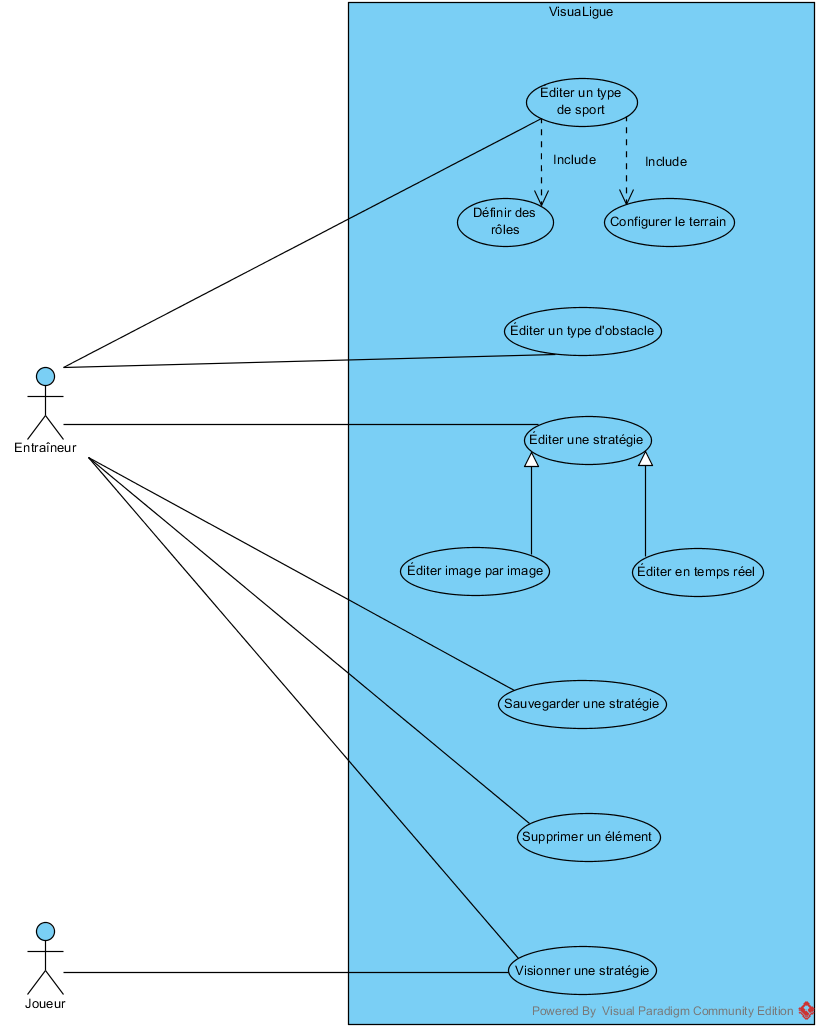
\includegraphics[scale=0.7]{fig/cas_utilisation_diag.png}
    \caption{Diagramme des cas d'utilisations}
    \label{fig:cas_utilisation_diag}
\end{figure}

\newpage

\section{Ajouter un type de sport}
\label{sec:ajouter_un_type_de_sport}

\subsection{Sc\'enario principal}
\label{sub:sc'enario_principal}
L'\textit{entra\^ineur} veut définir un sport pour l'application.
Il cr\'ee un sport, le nomme.
Ensuite il ajoute les \textit{r\^oles} du sport.
Finalement, il d\'efini un terrain en dessinant les lignes et en sp\'ecifiant les dimensions.

\subsection{Autres Situations}
\label{sub:autres_situations}
\begin{itemize}
    \item \textbf{Sport d\'ej\`a existant:} Si le sport existe d\'ej\`a dans l'application, un message d'avertissement appara\^it pour signaler que le sport existe d\'ej\`a. 
    L'entraîneur peut d\'ecider d'effacer ce qui \'etait dans le sport existant, d'enregister son sport sous un autre nom, ou d'oublier le sport cr\'e\'e. 
\end{itemize}

\section{Ajouter une stratégie}
\label{sec:ajouter_une_strategie}

\subsection{Pr\'erequis}
\label{sub:prerequis}

Le sport pour lequel l'entraîneur veut ajouter une stratégie doit exister dans l'application.

\subsection{Sc\'enario principal}
\label{sub:sc'enario_principal}

L'\textit{entraîneur} veut ajouter une nouvelle \textit{stratégie}.
Il choisi le sport pour la \textit{strat\'egie}.
Ensuite, pour chacun des joueurs, il leur assigne un \textit{r\^ole} et dessine leurs \textit{actions}.

\subsection{Autres Situations}
\label{sub:autres_situations}
\begin{itemize}
    \item \textbf{Sport d\'ej\`a existant:} Si la stratégie existe d\'ej\`a dans l'application, un message d'avertissement appara\^it pour signaler que celui-ci existe d\'ej\`a. 
    L'entraîneur peut d\'ecider d'effacer ce qui \'etait dans la stratégie existante, d'enregister sa stratégie sous un autre nom, ou d'oublier la stratégie cr\'e\'e. 
\end{itemize}

\section{Visualiser une stratégie}
\label{sec:visualiser_une_strategie}

\subsection{Pr\'erequis}
\label{sub:prerequis}
Il faut que la strat\'egie soit enregistr\'ee dans l'application pour que l'entraîneur puisse la visualiser.

\subsection{Sc\'enario principal}
\label{sub:sc'enario_principal}

L'\textit{entra\^ineur} s\'electionne la \textit{strat\'egie} \`a visualiser.
Il d\'ebute la visualisation et observe le d\'eroulement de la \textit{strat\'egie}.
Il peut mettre fin \`a la visualisation \`a tout moment.

\section{Exporter une stratégie}
\label{sec:exporter_une_strategie}

\subsection{Pr\'erequis}
\label{sub:prerequis}
Il faut que la strat\'egie soit enregistr\'ee dans l'application pour que l'entraîneur puisse l'exporter.

\subsection{Sc\'enario principal}
\label{sub:sc'enario_principal}

L' \textit{entra\^ineur} veut exporter une strat\'egie.
Il s\'electionne la strat\'egie et le format pour l'exportation.
Il applique l'exportation de la \textit{strat\'egie}.
